\documentclass{beamer}
\usepackage[utf8]{inputenc}
\usepackage[T1]{fontenc}
%\usepackage[french]{babel}
\usepackage{amsmath, amsfonts, amsthm, amssymb}
\usepackage{hyperref}


\title{GIT tutorial}
\author{Pauline Hubert and Nadia Lafrenière}
\date{FPSAC software days, July 2019}
\begin{document}
	\maketitle
	\begin{frame}{Motivation}
		PhD Comics
	\end{frame}
	\begin{frame}{What software to use? Pros and cons}
		\begin{tabular}{lp{0.35\linewidth}p{0.35\linewidth}}
%			\hline
			& Pros & Cons\\
			\hline
			Email & "Easy" to use & So many!\\
			\hline
			Overleaf & Many people can work at the same time & Only online, latex only\\
			\hline
			Dropbox & Easy to use & No two people can work at the same time, no version control\\
			\hline
			Git & Version control, automatic fusion of modifications, any file type & More difficult to start\\
%			\hline
		\end{tabular}
	\end{frame}
	\begin{frame}{What is Git?}
		Git is a version control software. \newline
		
		\begin{itemize}
			\item It keeps track of every modifications.
			\item You can go back in time to a previous version.
			\item It allows many people to work in parallel.
		\end{itemize}	
	\end{frame}
	\begin{frame}{Online servers for Git}
		Store your data somewhere. \newline 
			\begin{itemize}
				\item Local : on your computer.
				\item Online servers : Github, Bitbucket, GitLab, University server, etc. \newline
			\end{itemize}
		If you use an online server, you will also have a local version on your computer. If you want to work with other people, you have to use a server. 
	\end{frame}
	\begin{frame}{Now that you are convinced... Installation}
		\begin{itemize}
			\item Linux : Type in shell \texttt{sudo apt install git}
			\item MacOS : Go to \url{git-scm.com/download/mac}
			\item Windows : Go to \url{gitforwindows.com}
		\end{itemize}
	\end{frame}
	\begin{frame}[fragile]{Configuration}
	To share code, you need to identify yourself:
	\begin{verbatim}
		$ git config --global user.name "John Doe"
		$ git config --global user.email "john.doe@email.com"
	\end{verbatim}
	\end{frame}

	\begin{frame}{What's happening?}
		git status
	\end{frame}
	\begin{frame}[fragile]{First steps: Creating a folder and initializing}
		Two ways to start a new project : 
		\begin{itemize}
			\item Use an existant project. 
			\item Create a new project on Github and clone it. \newline
		\end{itemize}
	
		If your already have a project.
		\begin{enumerate}
		\item  In the directory containing your files run the command 
		\texttt{git init}.
		
		\item  Then you need to put your files on Github. For that, create a new \emph{empty} repository on Github and follow the instructions.
		
		The commands you will need are 
		\begin{verbatim}
			$ git remote add origin REPO_URL
			$ git push -u origin master
		\end{verbatim}
		
		\end{enumerate}   
	\end{frame}
	\begin{frame}{Getting code : cloning}
		contenu...
	\end{frame}
	\begin{frame}[fragile]{Modifications}
		Once you have worked on your code/text, you will want to save the modifications. \newline
		
		To select the (new or old) files that will be added to the modification use the command
		\begin{verbatim}
			$ git add FILE_NAMES
		\end{verbatim}
	\end{frame}
	\begin{frame}[fragile]{Modifications}	
		To save modifications, use the command \texttt{git commit}. \newline 
		
		Each time you made a commit, a text editor appears in your terminal and you have to write a short comment to describe your modifications. \newline
		
		If you modified only on files that were already in the git repository you can also list the files directly in the commit command. 
		\begin{verbatim}
		$ git commit FILE_NAMES
		\end{verbatim}
		
		Two usefull options : \texttt{git commit -OPTS}
		
		\texttt{-a} allows you to save all the modified files with the same comment.
		 
		\texttt{-m "Comment"} allows you to directly write your commit message in the command. 		
	\end{frame}
	\begin{frame}[fragile]{Sharing modifications}
		For the moment, all your modifications are only saved in your local copy of your project. 
		
		After committed, you may want to share your modifications by adding them in the online repository. The command for that is 
		
		\begin{verbatim}
		$ git push
		\end{verbatim}
		
		You may be asked to enter your username and password at this point.
		
		You don't have to push every time you commit. You can push several commits at once. 
	\end{frame}
	\begin{frame}[fragile]{Getting updated code \& solving conflicts}
		If you are working with other people, to obtain the updated version of the project use 
		\begin{verbatim}
		$ git pull
		\end{verbatim}
		
		\textit{"What if one of my collaborator worked at the same time as me?"}
		
		If this happens you will get an error message when you try to push. Then read and follow the instructions. 
	\end{frame}
	\begin{frame}{Compare different versions}
		DIFF (meld)
	\end{frame}
	\begin{frame}[fragile]{Branches}
		\footnotesize{Image from Bitbucket web site} \vspace{-.5cm}
		\begin{figure}[h]
			\centering
			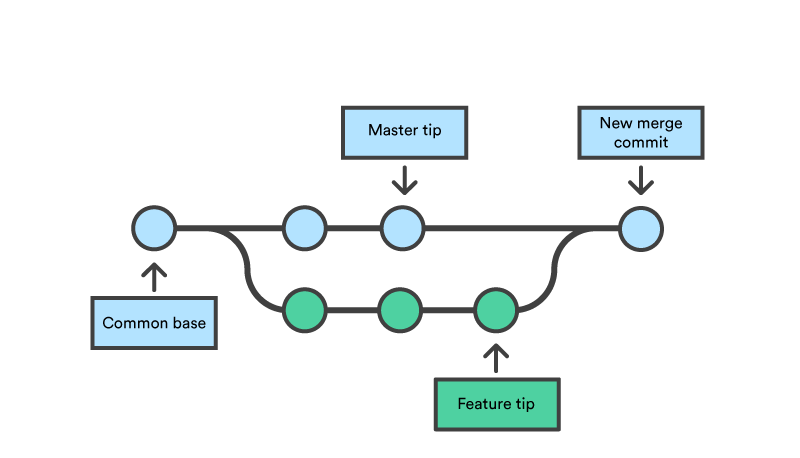
\includegraphics[scale=.3]{branch.png}
		\end{figure}
		
		Create a new branch : \texttt{\$ git branch BRANCH\_NAME}
		
		Navigate between branches : \texttt{\$ git checkout BRANCH\_NAME}
		
		Merge branches : \texttt{\$ git merge BRANCH\_NAME}
	\end{frame}
	\begin{frame}{Conclusion/Moral}
	Read the comments ! \newline
	
	References :
	\begin{itemize}
		\item Software Carpentry : \url{http://swcarpentry.github.io/git-novice/}
		\item Bitbucket :  \url{https://www.atlassian.com/git/tutorials/learn-git-with-bitbucket-cloud}
		\item Github : \url{https://guides.github.com/introduction/git-handbook/}
	\end{itemize}

	~

	Cheatsheets : 
	\begin{itemize}
		\item  Software Capentry : \url{http://swcarpentry.github.io/git-novice/reference}
		\item Github : \url{https://github.github.com/training-kit/downloads/github-git-cheat-sheet.pdf}
	\end{itemize}
	\end{frame}
	\begin{frame}
		Your turn
	\end{frame}	
\end{document}